\documentclass[conference]{IEEEtran}
\IEEEoverridecommandlockouts
% The preceding line is only needed to identify funding in the first footnote. If that is unneeded, please comment it out.
\usepackage{cite}
\usepackage{amsmath,amssymb,amsfonts}
\usepackage{algorithmic}
\usepackage{graphicx}
\usepackage{textcomp}
\usepackage{xcolor}
\def\BibTeX{{\rm B\kern-.05em{\sc i\kern-.025em b}\kern-.08em
    T\kern-.1667em\lower.7ex\hbox{E}\kern-.125emX}}
\begin{document}

\title{A comparison between LSTM and GRU for Deep Recurrent Q-Learning}

\author{\IEEEauthorblockN{ Erick D. Tornero Tenorio }
\IEEEauthorblockA{
\textit{San Pablo Catholic University}\\
Arequipa, Peru \\
erickdeivy01@gmail.com}
\and
\IEEEauthorblockN{ Victor Flores Benites }
\IEEEauthorblockA{
\textit{San Pablo Catholic University}\\
Arequipa, Peru  \\
victor.flores@ucsp.edu.pe}
}

\maketitle

\begin{abstract}
Since some applications in reinforcement learning require long term memory. Some architectures propose to add a recurrent layer with LSTM cells, the ability to remember more with these architectures is a consequence of the performance improvements shown in some Atari-2600 games such as Frostbite, where it is necessary to remember the way home after completing a certain score, this compared to a typical DQN. In the present paper we propose to use GRU cells which are easier to train, in the recurrent layer of a DRQN instead LSTM cells.
\end{abstract}


\begin{IEEEkeywords}
DQN, LSTM, GRU, reinforcement learning
\end{IEEEkeywords}

\section{Introduction}

Reinforcement learning is a machine learning inspired by behavioral psychology, whose objective is to determine what actions an agent should choose in a given environment in order to maximize some compensation.The agent perceives a finite set of different states $S$ in its environment, and has a finite set of actions $A$ to interact with it.Time advances discreetly, and at each instant of time $t$ the agent perceives a specific state, st, selects a possible action, $a_t$, and execute it, obtaining a new status, $s_{t+1} = a_t(s_t)$.
The environment responds to the action of the agent by a reward $r(s_t,a_t)$.
The goal of reinforcement learning is to extract what actions should be chosen in the different states to maximize the reward. For this, it looks for that the agent learns a policy, that formally is a relation between states and actions to take $S \times A$.

There are several methods of implementing these learning processes, where Q-Learning is a prominent method
In the Q Learning algorithm, the Q value of a pair (state, action) contains the sum of all these possible rewards. The problem is that this sum could be infinite in case there is no terminal state to reach and, in addition, we may not want to give the same weight to immediate rewards as to future rewards, in which case use is made of what is called an accumulated reinforcement with discount: future rewards are multiplied by a factor $\gamma \in [0,1] $ so that the higher this factor, the more influence future rewards have on the Q value of the pair analyzed. Formally:

\begin{equation}
    Q(s_t,a_t)=r(s_t,a_t) + \gamma \max a_{t+1}Q(s_{t+1},a_{t+1})
\end{equation}



LSTM is the first neural network architecture that introduces the concept of memory cell \cite{b5}.
The memory cell can retain its value for a short or long period of time as a function of its inputs, which allows the cell to remember important information calculated in previous stages.
The LSTM memory cell contains three gates that control how information flows inside or outside the cell. The gateway controls when new information can enter memory. The door of forgetfulness controls when a part of the information is forgotten, which allows the cell to remember new data. Finally, the exit door controls when the information that is contained in the cell is used in the result of the cell.

GRU was presented as a simplification of the LSTM.
This model has two doors, omitting the exit door that is present in the LSTM model.
The GRU includes two doors: an update door and a reset door. The update gate indicates how much of the contents of the previous cells must be maintained. The reset door defines how to incorporate the new entry with the previous contents of the cell.
For many applications, the GRU has a performance similar to that of LSTM, but being simpler has less weighting and faster execution.
The GRU is simpler than the LSTM, it can be trained more quickly and it can be more efficient in its execution. However, LSTM can store more information, which can provide better results.

Our experiments is build over Atari Learning Enviroment (ALE) \cite{b3} which serve us as an evaluation platform for our algorithm and allow us to compare with DRQN proposed by Hausknecht et al. 2015 \cite{b2}.



\section{Methods}

Using three DQN architectures. A classic DQN is implemented (Figure \ref{dqn}). Pre-processing cuts the frames obtained from the environment to $160\times160$ image. Then, the image is sub-sampled at $84\times84$ and image is transformed to scale gray. Classic DQN architecture includes three convolutional layers and two fully-connect layers (Figure 1). Output layer size depends on the number of actions in the game. 

\begin{figure}[htbp]
\centerline{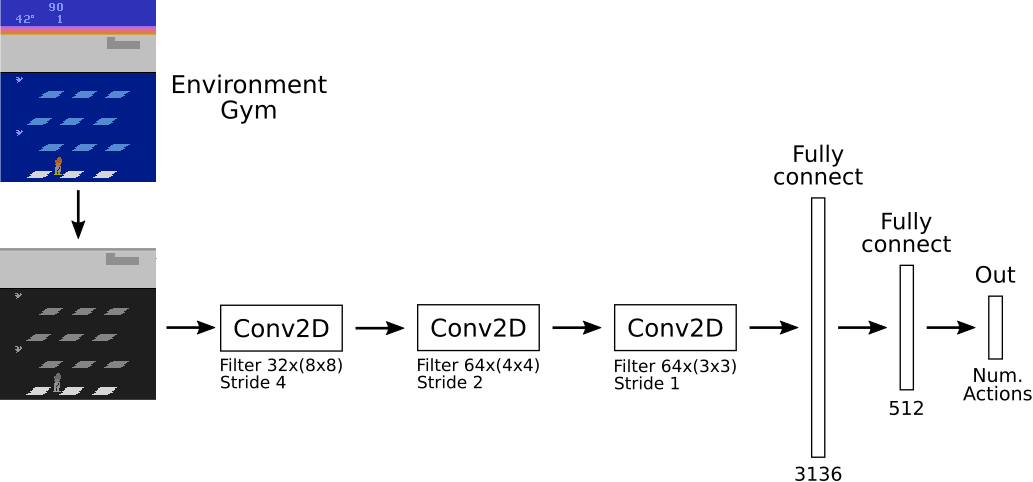
\includegraphics[width=\linewidth]{images/DQN.png}}
\caption{Example of a figure caption.}
\label{dqn}
\end{figure}

DRQN (Recurrent DQN) used the preprocessing method of DQN. The architecture includes three convolutional layers, one LSTM layer (512 cells), and one fully-connect layer (Figure \ref{drqn}). The hidden states of LSTM are input from fully-connect layer.

\begin{figure}[htbp]
\centerline{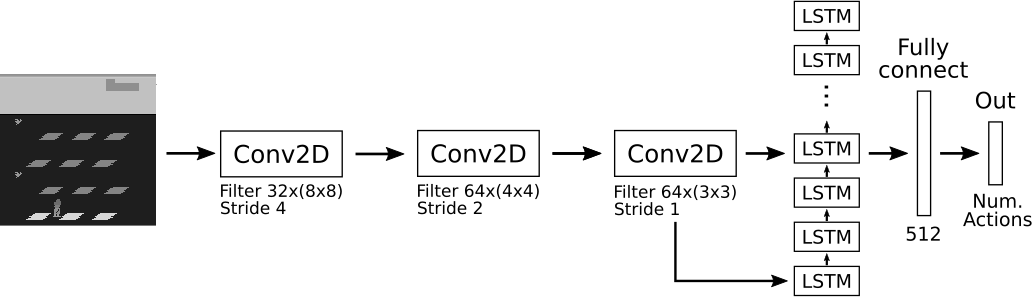
\includegraphics[width=\linewidth]{images/DRQN.png}}
\caption{Example of a figure caption.}
\label{drqn}
\end{figure}

We created a variant of DRQN, changing the LSTM cells to GRU. We call this method DGRQN. The architecture includes three convolutional layers, one GRU layer (512 cells), and one fully-connect layer (Figure \ref{dgrqn}). The hidden states of GRU are input from fully-connect layer.

\begin{figure}[htbp]
\centerline{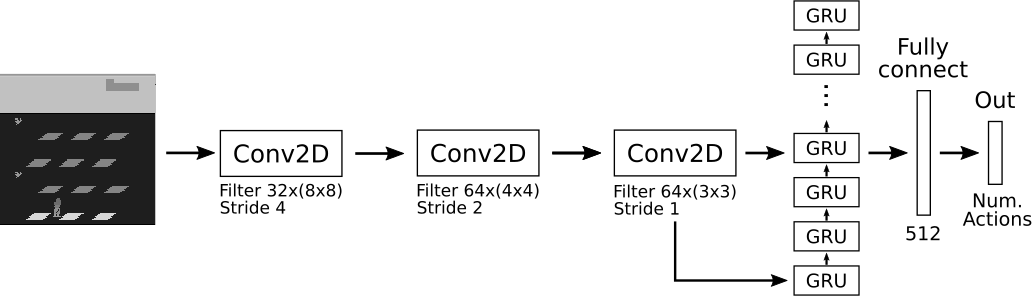
\includegraphics[width=\linewidth]{images/DGQN.png}}
\caption{Example of a figure caption.}
\label{dgrqn}
\end{figure}

All the architectures have as parameters:

\begin{itemize}
\item Learning rate method: RMSProp optimizer (learning rate 0.00025).
\item $\epsilon=[1 .. 0.02]$ ($\epsilon$ decay in 1000000 episodes).
\item Replay memory size: 800000.
\item Discount factor $\gamma = 0.99$
\end{itemize}



\section{Results}

We test the architecture in three diferent games, Enduro, Break-out and Frostbite with 10000000 (10 millions) of episodes.

Game Tested:
Enduro
\begin{figure}[htbp]
\centerline{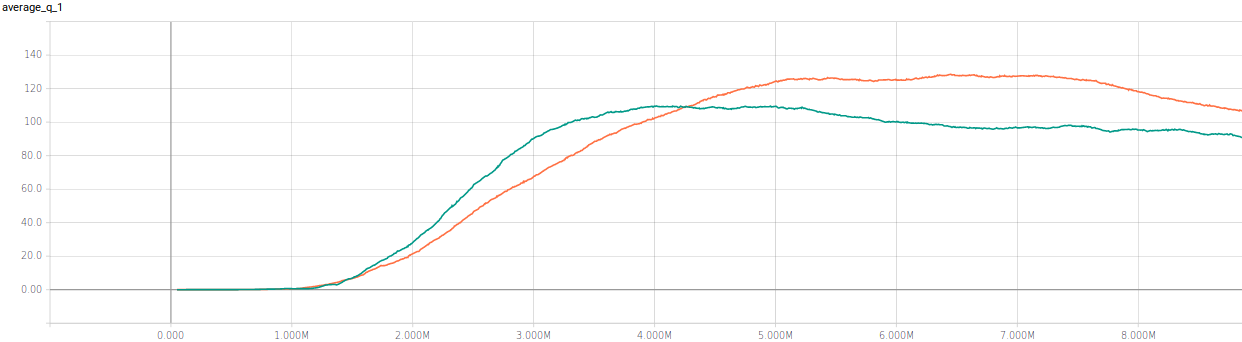
\includegraphics[width=\linewidth]{images/enduro-averQ-drqn-or-dgruqn-gr.png}}
\caption{Average Q Value Enduro, Orange DRQN, Green Our method.}
\label{enduro-q}
\end{figure}

\begin{figure}[htbp]
\centerline{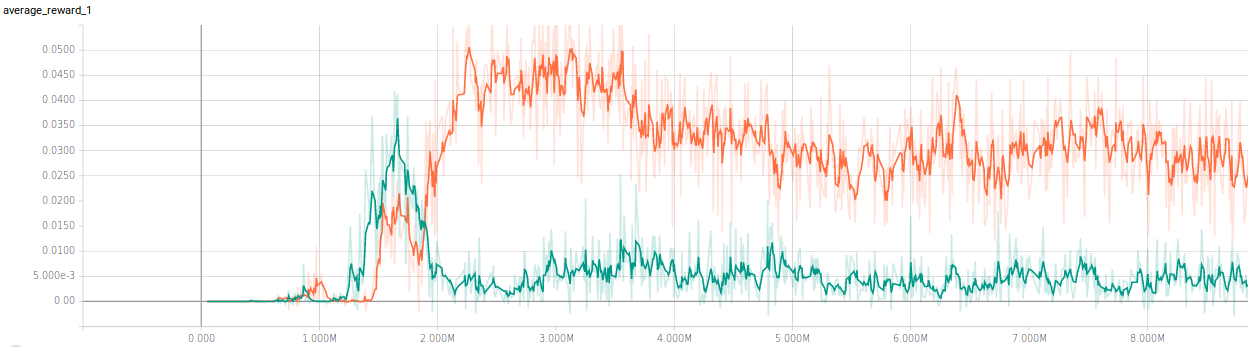
\includegraphics[width=\linewidth]{images/enduro-av-rew-drqn-or-dgruqn-gr.png}}
\caption{Average Reward Enduro, Orange DRQN, Green Our method.}
\label{enduro-r}
\end{figure}

Breakout:

\begin{figure}[htbp]
\centerline{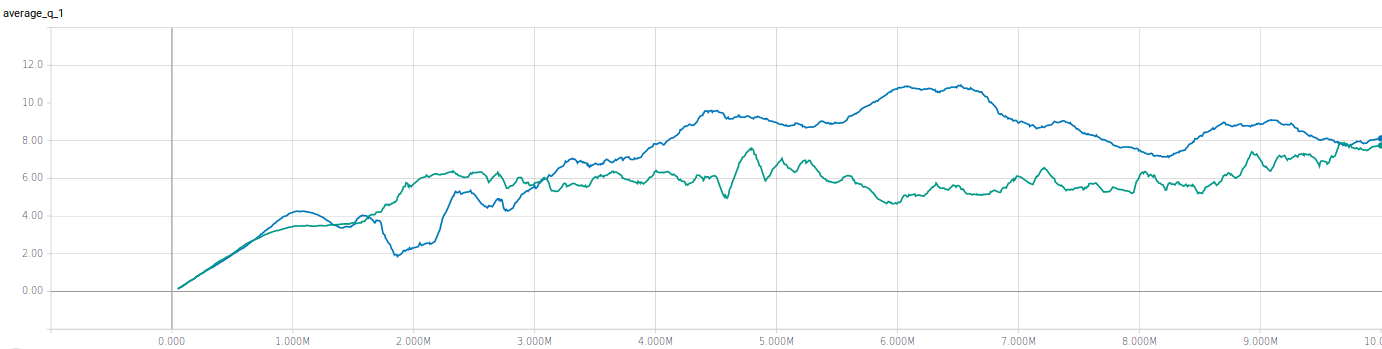
\includegraphics[width=\linewidth]{images/breakout-avQ-drqb-bl-dgruqn-gr.png}}
\caption{Average Q-value Breakout, Blue DRQN, Green Our method.}
\label{breakout-q}
\end{figure}

\begin{figure}[htbp]
\centerline{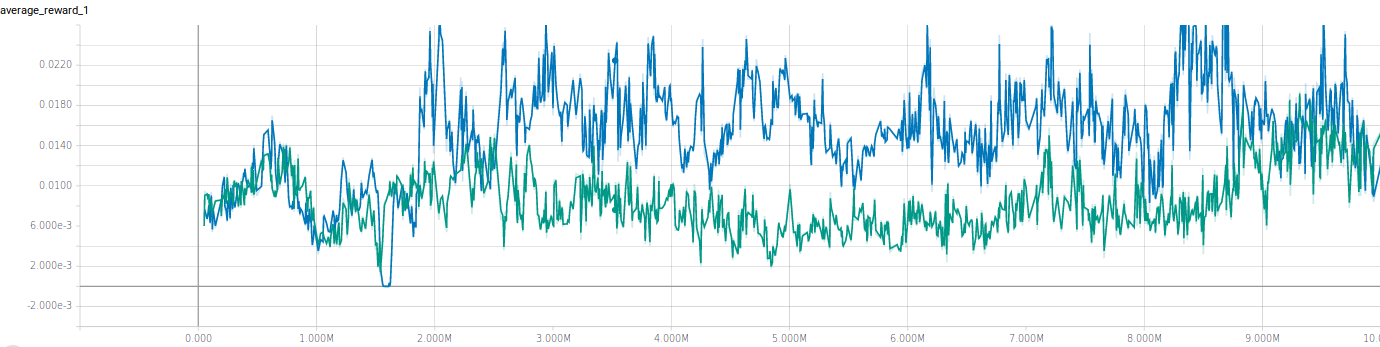
\includegraphics[width=\linewidth]{images/breakout-av-rew-drqn-bl-dgruqn-gr.png}}
\caption{Average Reward Breakout, Blue DRQN, Green Our method.}
\label{breakout-r}
\end{figure}

\section{Conclusions}

In Fig. \ref{enduro-q} and \ref{breakout-q} an small  improvement in the rising time, but in two cases our method the Q-values and the average reward is less than a tipical DRQN, this may be becouse an GRU is less robust than LSTM.



\begin{thebibliography}{00}
\bibitem{b1} V. Mnih, ``Playing Atari with Deep Reinforcement Learning``. In NIPS Deep Learning Workshop 2013.
\bibitem{b2} M. Hausknecht and Peter Stone, ``Deep Recurrent Q-Learning for Partially Observable MDPs``. In AAAI Fall Symposium Series 2015.
\bibitem{b3} M. Bellemare, Y. Naddaf, J. Veness and M. Bowling, ``The arcade learning enviroment. An evaluation platform for general agents``. In Journal of Artificial Intelligence Research, 47:253-279, 2013.
\bibitem{b4} Richard Sutton and Andrew Barto. ``Reinforcement Learning: An Introduction``. MIT Press, 1998.
\bibitem{b5} Hochreiter and Schmidhuber. ``Long short-term memory``. Neural Comput. 9(8):1735-1780.
\end{thebibliography}



\end{document}

